% Options for packages loaded elsewhere
\PassOptionsToPackage{unicode}{hyperref}
\PassOptionsToPackage{hyphens}{url}
\PassOptionsToPackage{dvipsnames,svgnames,x11names}{xcolor}
\documentclass[
  10pt,
  fontset=fandol]{ctexart}
\usepackage{xcolor}
\usepackage[margin=16mm]{geometry}
\usepackage{amsmath,amssymb}
\setcounter{secnumdepth}{-\maxdimen} % remove section numbering
\usepackage{iftex}
\ifPDFTeX
  \usepackage[T1]{fontenc}
  \usepackage[utf8]{inputenc}
  \usepackage{textcomp} % provide euro and other symbols
\else % if luatex or xetex
  \usepackage{unicode-math} % this also loads fontspec
  \defaultfontfeatures{Scale=MatchLowercase}
  \defaultfontfeatures[\rmfamily]{Ligatures=TeX,Scale=1}
\fi
\usepackage{lmodern}
\ifPDFTeX\else
  % xetex/luatex font selection
\fi
% Use upquote if available, for straight quotes in verbatim environments
\IfFileExists{upquote.sty}{\usepackage{upquote}}{}
\IfFileExists{microtype.sty}{% use microtype if available
  \usepackage[]{microtype}
  \UseMicrotypeSet[protrusion]{basicmath} % disable protrusion for tt fonts
}{}
\makeatletter
\@ifundefined{KOMAClassName}{% if non-KOMA class
  \IfFileExists{parskip.sty}{%
    \usepackage{parskip}
  }{% else
    \setlength{\parindent}{0pt}
    \setlength{\parskip}{6pt plus 2pt minus 1pt}}
}{% if KOMA class
  \KOMAoptions{parskip=half}}
\makeatother
\usepackage{longtable,booktabs,array}
\newcounter{none} % for unnumbered tables
\usepackage{calc} % for calculating minipage widths
% Correct order of tables after \paragraph or \subparagraph
\usepackage{etoolbox}
\makeatletter
\patchcmd\longtable{\par}{\if@noskipsec\mbox{}\fi\par}{}{}
\makeatother
% Allow footnotes in longtable head/foot
\IfFileExists{footnotehyper.sty}{\usepackage{footnotehyper}}{\usepackage{footnote}}
\makesavenoteenv{longtable}
\usepackage{graphicx}
\makeatletter
\newsavebox\pandoc@box
\newcommand*\pandocbounded[1]{% scales image to fit in text height/width
  \sbox\pandoc@box{#1}%
  \Gscale@div\@tempa{\textheight}{\dimexpr\ht\pandoc@box+\dp\pandoc@box\relax}%
  \Gscale@div\@tempb{\linewidth}{\wd\pandoc@box}%
  \ifdim\@tempb\p@<\@tempa\p@\let\@tempa\@tempb\fi% select the smaller of both
  \ifdim\@tempa\p@<\p@\scalebox{\@tempa}{\usebox\pandoc@box}%
  \else\usebox{\pandoc@box}%
  \fi%
}
% Set default figure placement to htbp
\def\fps@figure{htbp}
\makeatother
\setlength{\emergencystretch}{3em} % prevent overfull lines
\providecommand{\tightlist}{%
  \setlength{\itemsep}{0pt}\setlength{\parskip}{0pt}}
\usepackage{amsmath,amssymb,mathtools,needspace}
\xeCJKDeclareCharClass{CJK}{"2032,"0400->"04FF,"2160->"216B,"2460->"2473,"25A0,"25C7,"25CB,"25CF}
\IfFontExistsTF{Arial Unicode MS}{\xeCJKsetup{AutoFallBack=true}\setCJKfallbackfamilyfont{\CJKrmdefault}{Arial Unicode MS}}{}
\setcounter{secnumdepth}{0}
\setlength{\emergencystretch}{2em}
\allowdisplaybreaks
\usepackage{bookmark}
\IfFileExists{xurl.sty}{\usepackage{xurl}}{} % add URL line breaks if available
\urlstyle{same}
\hypersetup{
  pdftitle={Newton 法},
  colorlinks=true,
  linkcolor={Maroon},
  filecolor={Maroon},
  citecolor={Blue},
  urlcolor={Blue},
  pdfcreator={LaTeX via pandoc}}

\title{Newton 法}
\author{}
\date{}

\begin{document}
\maketitle

\subsection{6.3 Newton 法}\label{newton-ux6cd5}

\subsubsection{6.3.1 Newton 公式}\label{newton-ux516cux5f0f}

对于方程 \(f(x)=0\)，为要应用迭代法，必须先将它改写成 \(x=\varphi(x)\) 的形式，即需要针对所给的函数 \(f(x)\) 构造合适的迭代函数 \(\varphi(x)\)。

迭代函数 \(\varphi(x)\) 可以是多种多样的。例如，可令 \(\varphi(x)=x+f(x)\)，这时相应的迭代公式是

\href{../../source-images/pdf-163.jpeg}{原页}

\[
x_{k+1}=x_k+f(x_k).
\tag{6.3.1}
\]

一般来说，这种迭代公式不一定收敛，或者收敛的速度缓慢。

运用前述加速技巧，对于迭代过程（6.3.1），其加速公式（6.2.10）具有以下形式：

\[
\begin{cases}
\bar{x}_{k+1}=x_k+f(x_k),\\
x_{k+1}=\bar{x}_{k+1}+\dfrac{L}{1-L}(\bar{x}_{k+1}-x_k).
\end{cases}
\]

记 \(M=L-1\)，上面两个式子可以合并写成

\[
x_{k+1}=x_k-\frac{f(x_k)}{M}.
\]

这种迭代公式通常称为简化的 Newton 公式，其相应的迭代函数是

\[
\varphi(x)=x-\frac{f(x)}{M}.
\tag{6.3.2}
\]

需要注意的是，由于 \(L\) 是 \(\varphi'(x)\) 的估计值，而 \(\varphi(x)=x+f(x)\)，这里的 \(M=L-1\) 实际上是 \(f'(x)\) 的估计值。如果用 \(f'(x)\) 代替式（6.3.2）中的 \(M\)，则得到如下形式的迭代函数：

\[
\varphi(x)=x-\frac{f(x)}{f'(x)},
\]

其相应的迭代公式

\[
x_{k+1}=x_k-\frac{f(x_k)}{f'(x_k)}
\tag{6.3.3}
\]

就是著名的 Newton 公式。

\subsubsection{6.3.2 Newton 法的几何解释}\label{newton-ux6cd5ux7684ux51e0ux4f55ux89e3ux91ca}

对于方程 \(f(x)=0\)，如果 \(f(x)\) 是线性函数，则对它求根是容易的。Newton 法实质上是一种线性化方法，其基本思想是将非线性方程 \(f(x)=0\) 逐步归结为某种线性方程来求解。

设已知方程 \(f(x)=0\) 有近似根 \(x_k\)，将函数 \(f(x)\) 在点 \(x_k\) 展开，有

\[
f(x)\approx f(x_k)+f'(x_k)(x-x_k),
\]

于是方程 \(f(x)=0\) 可近似地表示为

\[
f(x_k)+f'(x_k)(x-x_k)=0.
\tag{6.3.4}
\]

这是个线性方程，记其根为 \(x_{k+1}\)，则 \(x_{k+1}\) 的计算公式就是 Newton 公式（6.3.3）。

Newton 法有明显的几何解释。方程 \(f(x)=0\) 的根 \(x^*\) 可解释为曲线 \(y=f(x)\) 与 \(x\) 轴的交点的横坐标（见图 6.3）。设 \(x_k\) 是根 \(x^*\) 的某个近似值，过曲

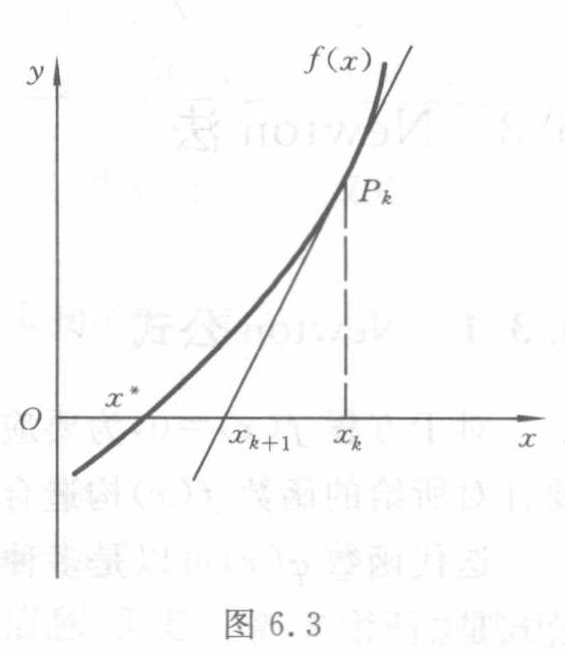
\includegraphics[width=0.85\linewidth,height=\textheight,keepaspectratio,alt={图 6.3 原扫描裁切}]{../assets/ch06/fig-6.3.png}

图 6.3

图意（agent 整理）：曲线 \(f(x)\) 在 \(P_k\) 处的切线与 \(x\) 轴相交，其交点横坐标是 \(x_{k+1}\)。全部标签为 \(x,\allowbreak y,\allowbreak O,\allowbreak x^*,\allowbreak x_{k+1},\allowbreak x_k,\allowbreak P_k,\allowbreak f(x)\)。

\href{../../source-images/pdf-164.jpeg}{原页}

线 \(y=f(x)\) 上横坐标为 \(x_k\) 的点 \(P_k\) 引切线，并将该切线与 \(x\) 轴的交点的横坐标 \(x_{k+1}\) 作为 \(x^*\) 的新的近似值。注意到切线方程为

\[
y=f(x_k)+f'(x_k)(x-x_k).
\]

这样求得的值 \(x_{k+1}\) 必满足式（6.3.4），从而就是 Newton 公式（6.3.3）的计算结果。由于这种几何背景，Newton 法亦称切线法。

\subsubsection{6.3.3 Newton 法的局部收敛性}\label{newton-ux6cd5ux7684ux5c40ux90e8ux6536ux655bux6027}

对于一种迭代过程，为了保证它是有效的，需要肯定它的收敛性，同时考察它的收敛速度。所谓迭代过程的收敛速度，是指在接近收敛的过程中迭代误差的下降速度。

\textbf{定义 6.2} 设迭代过程 \(x_{k+1}=\varphi(x_k)\) 收敛于方程 \(x=\varphi(x)\) 的根 \(x^*\)，如果迭代误差 \(e_k=x_k-x^*\) 当 \(k\to\infty\) 时成立下列渐近关系式：

\[
\frac{e_{k+1}}{e_k^p}\to C\quad(C\ne0\text{ 为常数}),
\]

则称该迭代过程是 \(p\) 阶收敛的。特别地，\(p=1\) 时称为线性收敛，\(p>1\) 时称为超线性收敛，\(p=2\) 时称为平方收敛。

\textbf{定理 6.3} 对于迭代过程 \(x_{k+1}=\varphi(x_k)\)，如果 \(\varphi^{(p)}(x)\) 在所求根 \(x^*\) 的邻近连续，并且

\[
\begin{cases}
\varphi'(x^*)=\varphi''(x^*)=\cdots=\varphi^{(p-1)}(x^*)=0,\\
\varphi^{(p)}(x^*)\ne0,
\end{cases}
\tag{6.3.5}
\]

则该迭代过程在点 \(x^*\) 邻近是 \(p\) 阶收敛的。

\textbf{证明} 由于 \(\varphi'(x^*)=0\)，据定理 6.2 立即可以断定迭代过程 \(x_{k+1}=\varphi(x_k)\) 具有局部收敛性。

再将 \(\varphi(x_k)\) 在根 \(x^*\) 处展开，利用条件（6.3.5），则有

\[
\varphi(x_k)=\varphi(x^*)+\frac{\varphi^{(p)}(\zeta)}{p!}(x_k-x^*)^p.
\]

注意到

\[
\varphi(x_k)=x_{k+1},\quad\varphi(x^*)=x^*,
\]

由上式得

\[
x_{k+1}-x^*=\frac{\varphi^{(p)}(\zeta)}{p!}(x_k-x^*)^p,
\]

因此对于迭代误差，有 \(\dfrac{e_{k+1}}{e_k^p}\to\dfrac{\varphi^{(p)}(x^*)}{p!}\)。这表明迭代过程 \(x_{k+1}=\varphi(x_k)\) 确实是 \(p\) 阶收敛的。证毕。

由上述定理可知，迭代过程的收敛速度依赖于迭代函数 \(\varphi(x)\) 的选取。如果当 \(x\in[a,b]\) 时 \(\varphi'(x)\ne0\)，则该迭代过程只可能是线性收敛的。

对于 Newton 公式（6.3.3），其迭代函数为

\href{../../source-images/pdf-165.jpeg}{原页}

\[
\varphi(x)=x-\frac{f(x)}{f'(x)},\quad\varphi'(x)=\frac{f(x)f''(x)}{[f'(x)]^2}.
\]

假定 \(x^*\) 是 \(f(x)\) 的一个单根，即 \(f(x^*)=0,f'(x^*)\ne0\)，则由上式知 \(\varphi'(x^*)=0\)，于是依据定理 6.3 可以断定，Newton 法在根 \(x^*\) 的邻近是平方收敛的。

\textbf{例 6.7} 用 Newton 法解方程

\[
x\mathrm{e}^x-1=0.
\tag{6.3.6}
\]

\textbf{解} 这里 Newton 公式为 \(x_{k+1}=x_k-\dfrac{x_k-\mathrm{e}^{-x_k}}{1+x_k}\)，取迭代初值 \(x_0=0.5\)，迭代结果列于表 6.7 中。

表 6.7

{\def\LTcaptype{none} % do not increment counter
\begin{longtable}[]{@{}ll@{}}
\toprule\noalign{}
\(k\) & \(x_k\) \\
\midrule\noalign{}
\endhead
\bottomrule\noalign{}
\endlastfoot
\(0\) & \(0.5\) \\
\(1\) & \(0.571\,02\) \\
\(2\) & \(0.567\,16\) \\
\(3\) & \(0.567\,14\) \\
\end{longtable}
}

所给方程（6.3.6）实际上是方程 \(x=\mathrm{e}^{-x}\) 的等价形式。比较例 6.7 与例 6.5 的计算结果可以看出，Newton 法的收敛速度是很快的。

下面列出 Newton 法的计算步骤：

\textbf{步 1} 准备。选定初始近似值 \(x_0\)，计算 \(f_0=f(x_0),f'_0=f'(x_0)\)。

\textbf{步 2} 迭代。按公式 \(x_1=x_0-f_0/f'_0\) 迭代一次，得新的近似值 \(x_1\)，计算

\[
f_1=f(x_1),\quad f'_1=f'(x_1).
\]

\textbf{步 3} 控制。如果 \(x_1\) 满足 \(|\delta|<\varepsilon_1\) 或 \(|f_1|<\varepsilon_2\)，则终止迭代，以 \(x_1\) 作为所求的根；否则转步 4。此处 \(\varepsilon_1,\varepsilon_2\) 是允许误差，而

\[
\delta=\begin{cases}
|x_1-x_0|,&\text{当 }|x_1|<C\text{ 时},\\
\dfrac{|x_1-x_0|}{|x_1|},&\text{当 }|x_1|\geqslant C\text{ 时},
\end{cases}
\]

其中 \(C\) 是取绝对误差或相对误差的控制常数，一般可取 \(C=1\)。

\textbf{步 4} 修改。如果迭代次数达到预先指定的次数 \(N\) 或者 \(f'_1=0\)，则方法失败，否则以 \((x_1,f_1,f')\) 代替 \((x_0,f_0,f'_0)\) 转步 2 继续迭代。

\subsubsection{6.3.4 Newton 法应用举例}\label{newton-ux6cd5ux5e94ux7528ux4e3eux4f8b}

对于给定正数 \(a\)，应用 Newton 法解二次方程 \(x^2-a=0\)，可导出求开方值 \(\sqrt{a}\) 的计算程序

\[
x_{k+1}=\frac{1}{2}\left(x_k+\frac{a}{x_k}\right).
\tag{6.3.7}
\]

下面证明这种迭代公式对于任意初值 \(x_0>0\) 都是收敛的。

事实上，对式（6.3.7）施行配方手续，易知

\[
x_{k+1}-\sqrt{a}=\frac{1}{2x_k}(x_k-\sqrt{a})^2,\quad
x_{k+1}+\sqrt{a}=\frac{1}{2x_k}(x_k+\sqrt{a})^2.
\]

将以上两式相除得

\begin{quote}
校注（agent 补充）：原页步 4 的替换三元组印为 \((x_1,f_1,f')\)，第三项未印下标 \(1\)，转录保留原式。结合步 2 的定义及被替换的 \(f'_0\)，这里疑应为 \(f'_1\)。这是原扫描上的疑似漏印，非 OCR 改写；局部原图见 \href{../assets/ch06/detail-p165-step4.png}{步 4 裁切}。
\end{quote}

\begin{quote}
校注（agent 补充）：本页首段``单根''推出``平方收敛''的原文亦予保留。若按前页定义 6.2 要求精确收敛阶的极限常数非零，则还需 \(f''(x^*)\ne0\) 才能断言恰为二阶；在通常光滑性条件下，单根保证的是局部至少二阶收敛。例如 \(f(x)=x+x^3\) 在单根 \(0\) 附近的 Newton 迭代为 \(x_{k+1}=2x_k^3/(1+3x_k^2)\)，实际为三阶。这是原文收敛阶表述的适用条件说明。
\end{quote}

\href{../../source-images/pdf-166.jpeg}{原页}

\[
\frac{x_{k+1}-\sqrt{a}}{x_{k+1}+\sqrt{a}}=\left[\frac{x_k-\sqrt{a}}{x_k+\sqrt{a}}\right]^2.
\]

据此反复递推，有

\[
\frac{x_k-\sqrt{a}}{x_k+\sqrt{a}}=\left[\frac{x_0-\sqrt{a}}{x_0+\sqrt{a}}\right]^{2^k},
\tag{6.3.8}
\]

记 \(q=\dfrac{x_0-\sqrt{a}}{x_0+\sqrt{a}}\)，整理式（6.3.8），得

\[
x_k-\sqrt{a}=2\sqrt{a}\frac{q^{2^k}}{1-q^{2^k}}.
\]

对于任意 \(x_0>0\)，总有 \(|q|<1\)，故由上式推知，当 \(k\to\infty\) 时 \(x_k\to\sqrt{a}\)，即迭代过程恒收敛。

\textbf{例 6.8} 求 \(\sqrt{115}\)。

\textbf{解} 取初值 \(x_0=10\)，对 \(a=115\) 按式（6.3.7）迭代 3 次便得到精度为 \(10^{-6}\) 的结果（见表 6.8）。

表 6.8

{\def\LTcaptype{none} % do not increment counter
\begin{longtable}[]{@{}ll@{}}
\toprule\noalign{}
\(k\) & \(x_k\) \\
\midrule\noalign{}
\endhead
\bottomrule\noalign{}
\endlastfoot
\(0\) & \(10\) \\
\(1\) & \(10.750\,000\) \\
\(2\) & \(10.723\,837\) \\
\(3\) & \(10.723\,805\) \\
\(4\) & \(10.723\,805\) \\
\end{longtable}
}

由于式（6.3.7）对于任意初值 \(x_0>0\) 均收敛，并且收敛的速度很快，因此，可取确定的初值如 \(x_0=1\) 编制通用程序。用这个通用程序求 \(\sqrt{115}\)，也只要迭代 7 次便得到了上面的结果 \(10.723\,805\)。

再举一个例子。

对于给定的正数 \(a\)，应用 Newton 法于方程 \(1/x-a=0\)，可导出求 \(1/a\) 而不用除法的计算程序，即

\[
x_{k+1}=x_k(2-ax_k).
\]

这个算法有实际意义，早期设计电子计算机时，为节省硬件设备，曾运用这种技术避开除法操作的设置。

下面证明这一算法当初值 \(x_0\) 满足 \(0<x_0<2/a\) 时是收敛的。事实上，由于

\[
x_{k+1}-\frac{1}{a}=x_k(2-ax_k)-\frac{1}{a}=-a\left(x_k-\frac{1}{a}\right)^2,
\]

因而，对 \(r_k=1-ax_k\) 有递推公式 \(r_{k+1}=r_k^2\)。据此反复递推，有

\[
r_k=r_0^{2^k}.
\]

若初值满足 \(0<x_0<\dfrac{2}{a}\)，则对 \(r_0=1-ax_0\) 有 \(|r_0|<1\)。这时将有 \(r_k\to0\)，从而迭代收敛。

\subsubsection{6.3.5 Newton 下山法}\label{newton-ux4e0bux5c71ux6cd5}

前面已经讨论过 Newton 法的局部收敛性。一般来说，Newton 法的收敛性依赖

\href{../../source-images/pdf-167.jpeg}{原页}

于初值 \(x_0\) 的选取，如果 \(x_0\) 偏离所求的根 \(x^*\) 比较远，则 Newton 法可能发散。

例如，用 Newton 法求方程

\[
x^3-x-1=0,
\tag{6.3.9}
\]

在 \(x=1.5\) 附近的一个根 \(x^*\)。设取迭代初值 \(x_0=1.5\)，用 Newton 公式

\[
x_{k+1}=x_k-\frac{x_k^3-x_k-1}{3x_k^2-1}
\tag{6.3.10}
\]

计算，得

\[
x_1=1.347\,83,\quad x_2=1.325\,20,\quad x_3=1.324\,72.
\]

迭代三次得到的结果 \(x_3\) 有六位有效数字。

但是，如果改用 \(x_0=0.6\) 作为迭代初值，则依 Newton 公式（6.3.10）迭代一次得

\[
x_1=17.9.
\]

这个结果反而比 \(x_0=0.6\) 更偏离了所求的根 \(x^*=1.324\,72\)。

为了防止迭代发散，对迭代过程再附加一项要求，即具有单调性

\[
|f(x_{k+1})|<|f(x_k)|.
\tag{6.3.11}
\]

满足这项要求的算法称为下山法。

将 Newton 法与下山法结合起来使用，即可在下山法保证函数值稳定下降的前提下，用 Newton 法加快收敛速度。为此，将 Newton 法的计算结果 \(\bar{x}_{k+1}=x_k-\dfrac{f(x_k)}{f'(x_k)}\) 与前一步的近似值 \(x_k\) 适当加权平均作为新的改进值，即

\[
x_{k+1}=\lambda\bar{x}_{k+1}+(1-\lambda)x_k,
\tag{6.3.12}
\]

其中 \(\lambda\ (0<\lambda\leqslant1)\) 称为下山因子。在希望挑选下山因子时，希望使单调性条件（6.3.11）成立。

下山因子的选择是个逐步探索的过程。设从 \(\lambda=1\) 开始反复将 \(\lambda\) 减半进行试算，如果能定出值 \(\lambda\) 使单调性条件（6.3.11）成立，则称``下山成功''。与此相反，如果在上述过程中找不到使条件（6.3.11）成立的下山因子 \(\lambda\)，则称``下山失败''，这时需另选初值 \(x_0\) 重算。

\subsection{本节覆盖原页的校注记录}\label{ux672cux8282ux8986ux76d6ux539fux9875ux7684ux6821ux6ce8ux8bb0ux5f55}

下列记录按原页关联，含同页相邻小节的校注；计算时同时读取上文校注和完整原页。

\begin{itemize}
\tightlist
\item
  \texttt{ch06-E002}：原书 PDF 页 165
\item
  \texttt{ch06-E008}：原书 PDF 页 165
\end{itemize}

\end{document}
